\documentclass[a4paper,11pt]{article}
\usepackage{amsmath,amsthm,amsfonts,amssymb,amscd,amstext,vmargin,graphics,graphicx,tabularx,multicol} 
\usepackage[francais]{babel}
\usepackage[utf8]{inputenc}  
\usepackage[T1]{fontenc} 
\usepackage{pstricks-add,tikz,tkz-tab,variations}
\usepackage[autolanguage,np]{numprint} 
\usepackage{calc}
\usepackage{mathrsfs}

\setmarginsrb{1.5cm}{0.5cm}{1cm}{0.5cm}{0cm}{0cm}{0cm}{0cm} %Gauche, haut, droite, haut
\newcounter{numexo}
\newcommand{\exo}[1]{\stepcounter{numexo}\noindent{\bf Exercice~\thenumexo} : }
\reversemarginpar

\newcommand{\bmul}[1]{\begin{multicols}{#1}}
\newcommand{\emul}{\end{multicols}}

\renewcommand{\thesection}{\Roman{section}.}
	\renewcommand{\thesubsection}{\hspace{.5cm}\arabic{subsection}.}
	\renewcommand{\thesubsubsection}{\hspace{1cm}\alph{subsubsection})}

\newcounter{enumtabi}
\newcounter{enumtaba}
\newcommand{\q}{\textbf{\stepcounter{enumtabi} \theenumtabi)}  }
\newcommand{\qa}{\textbf{\stepcounter{enumtaba} \alph{enumtaba})} }
\newcommand{\initq}{\setcounter{enumtabi}{0}}
\newcommand{\initqa}{\setcounter{enumtaba}{0}}

\newcommand{\be}{\begin{enumerate}}
\newcommand{\ee}{\end{enumerate}}
\newcommand{\bi}{\begin{itemize}}
\newcommand{\ei}{\end{itemize}}
\newcommand{\bp}{\begin{pspicture*}}
\newcommand{\ep}{\end{pspicture*}}
\newcommand{\bt}{\begin{tabular}}
\newcommand{\et}{\end{tabular}}
\renewcommand{\tabularxcolumn}[1]{>{\centering}m{#1}} %(colonne m{} centrée, au lieu de p par défault) 
\newcommand{\tnl}{\tabularnewline}

\newcommand{\trait}{\noindent \rule{\linewidth}{0.2mm}}
\newcommand{\hs}[1]{\hspace{#1}}
\newcommand{\vs}[1]{\vspace{#1}}

\newcommand{\N}{\mathbb{N}}
\newcommand{\Z}{\mathbb{Z}}
\newcommand{\R}{\mathbb{R}}
\newcommand{\C}{\mathbb{C}}
\newcommand{\Dcal}{\mathcal{D}}
\newcommand{\Ccal}{\mathcal{C}}
\newcommand{\mc}{\mathcal}

\newcommand{\vect}[1]{\overrightarrow{#1}}
\newcommand{\ds}{\displaystyle}
\newcommand{\eq}{\quad \Leftrightarrow \quad}
\newcommand{\vecti}{\vec{\imath}}
\newcommand{\vectj}{\vec{\jmath}}
\newcommand{\Oij}{(O;\vec{\imath}, \vec{\jmath})}
\newcommand{\OIJ}{(O;I,J)}


\newcommand{\reponse}[1][1]{%
\multido{}{#1}{\makebox[\linewidth]{\rule[0pt]{0pt}{20pt}\dotfill}
}}

\newcommand{\titre}[5] 
% #1: titre #2: haut gauche #3: bas gauche #4: haut droite #5: bas droite
{
\noindent #2 \hfill #4 \\
#3 \hfill #5

\vspace{-1.6cm}

\begin{center}\rule{6cm}{0.5mm}\end{center}
\vspace{0.2cm}
\begin{center}{\Large{\textbf{#1}}}\end{center}
\begin{center}\rule{6cm}{0.5mm}\end{center}
}



\begin{document}
\pagestyle{empty}

\titre{Accompagnement  : Représenter un vecteur}{}{}{2nd}{}


\exo\\


\includegraphics[scale=1.9]{exo1accp3.eps} \\

\exo\\

\includegraphics[scale=1.7]{exo2accp3.eps} 

\bmul{2}
\exo\\
ABC est un triangle.\\
Représenter les points M, N, P et Q tels que :\\
$\overrightarrow{AM}=\overrightarrow{AB}+\overrightarrow{AC}$ \hspace*{0.75cm} $\overrightarrow{BN}=\overrightarrow{AC}+\overrightarrow{BA}$\\
$\overrightarrow{CP}=2\overrightarrow{AB}$ \hspace*{1.5cm} $\overrightarrow{AQ}=\overrightarrow{BC}+\overrightarrow{AC}$\\
\includegraphics[scale=1.9]{exo3accp3.eps} 


\columnbreak

\exo\\
ABC est un triangle.\\
Représenter les points M, N, P et Q tels que :\\
$\overrightarrow{AM}=2\overrightarrow{BC}$ \hspace*{2cm} $\overrightarrow{BN}=\dfrac{2}{3}\overrightarrow{AC}$ \\
$\overrightarrow{CP}=2\overrightarrow{AB}-\dfrac{1}{3}\overrightarrow{AC}$ \hspace*{1cm}  $\overrightarrow{AQ}=-\dfrac{4}{3}\overrightarrow{AC}$ \\
\includegraphics[scale=2]{exo4accp3.eps} 

\emul






\end{document}

